\lecmargin{1}

{\bf \large What is Complex Analysis?} The main object of study is a \cdef{holomorphic} function $f: G \to \cc$, where $G \subseteq \cc$. Namely, a function for which the limit
\[\lim_{h\to 0}\frac{f(z+h) - f(z)}{h}\]
exists and is finite on an open set; that is, a \cdef{complex\text{-}differentiable\  function} on an open set. As a set, $\cc = \rr^2$, so one can naively expect the theory to be similar to that of real analysis, in this case the behaviour of differentiable functions. Interestingly, the requirement of holomorphicity can yield results that have no counterpart in the real case.\\
\\
A prime example of this is \emph{Louiville's Theorem. Every bounded holomorphic function is constant.}

\medskip

\begin{discussion}
We begin with first addressing the existence and nature of $\cc$ itself. Let $\rr$ denote the (field of) real numbers. One immediately deduces that the equation
\begin{equation*}\label{imaginary}
x^2 + 1 = 0\tag{$*$}
\end{equation*}
has no solution in the real numbers. The (field of) complex numbers $\cc$ stems from our desire to find a set containing $\rr$ that extends the algebraic operations of addition and multiplication of real numbers and which contains not only solutions to the polynomial equation above but solutions to all polynomial equations.\\[0.5em]
Surprisingly enough, the construction amounts to defining a symbol $i$ that is a solution to (\ref{imaginary}) and then considering all expressions of the form
\[x + iy,\quad x,y \in \rr\]
\end{discussion}

\bigskip

\section{Part I. Preliminaries}
\subsection{Construction of the (field of) Complex Numbers}
%\begin{mdframed}[backgroundcolor=paleyellow,linewidth=1pt]
%\begin{center}
%\section*{\sc\Large Part I. Preliminaries}
%\end{center}
%\end{mdframed}
%
%\begin{mdframed}
%\begin{center}
%\subsection*{\Large Construction of the (field of) Complex Numbers}
%\end{center}
%\end{mdframed}

\begin{definition}[The set of Complex Numbers]
A \cdef{complex\ number} $z$ is simply an order pair $z \coloneqq (x,y)$ of real numbers. Thus, the set of all complex numbers is given by
\[\cc \coloneqq \rr^2 = \setp{(x,y)}{x,y\in \rr}\]
If $z = (x,y)$ is a complex number, then we call 
\[\Re z \coloneqq x \quad \text{and} \quad \Im z \coloneqq y\]
the \cdef{real} and \cdef{imaginary\ parts} of $z$ respectively.\\[0.5em]
Two complex numbers $z_1$ and $z_2$ are equal if and only if $\Re z_1 = \Re z_2$ and $\Im z_1 = \Im z_2$.\\
\\
If $\Re z = 0$ and $\Im z \neq 0$, we say that $z$ is \cdef{purely\ imaginary}. The set of purely imaginary complex numbers corresponds to the $y$-axis and is called the \cdef{imaginary\ axis} in $\cc$.
\end{definition}

\medskip

\begin{definition}[Binary Operations on $\cc$]
Let $z_1 = (x_1,y_1)$ and $z_2 = (x_2,y_2)$ be complex numbers. Then their \emph{sum} is
\[z_1 + z_2 = (x_1,y_1) + (x_2,y_2) \coloneqq (x_1 + x_2,y_1 + y_2)\]
and their \emph{product} is 
\[z_1 \cdot z_2 = (x_1,y_1) \cdot (x_2,y_2) \coloneqq (x_1x_2 - y_1y_2, x_1y_2 + x_2y_1)\]
\end{definition}

\medskip

\begin{proposition}
There exists a subset of $\cc$ that is algebraically indistinguishable from $\rr$.
\end{proposition}
\begin{proof}
Consider the set (the $x$-axis)
\[\rr \times \set{0} = \setp{(x,0)}{x\in \rr} \subseteq \cc.\]
There is a bijection
\[\phi:\rr \to \rr \times \set{0},\ x \mapsto (x,0).\]
Moreover, 
\begin{align*}
\phi(x) + \phi(y) &= (x,0) + (y,0) = (x+y,0) = \phi(x+y)\\[0.5em]
\phi(x)\cdot\phi(y) &= (x,0)\cdot (y,0) = (xy - 0\cdot 0,x\cdot 0 + y\cdot 0) = (xy,0) = \phi(xy)\\[-2.5em]
\end{align*}
\end{proof}
According to the proposition, the operations of addition and multiplication on complex numbers we have defined extend the operations of addition and multiplication of real numbers. We therefore call the $x$-axis, the \cdef{real\ axis}.

\medskip

\begin{discussion}
We identify each complex number $(x,0)$ with the corresponding real number $x$; more than that, abusing notation, we write
\[1 = (1,0)\quad \text{and} \quad (x,0) = x(1,0) = x\]
Now, define the \cdef{imaginary\ unit} $i \coloneqq (0,1)$. Then
\[i^2 = i\cdot i = (0,1)\cdot (0,1) = (0^2 - 1^2,1\cdot 0 + 1\cdot 0) = (-1,0) = -1.\]
Moreover, for any $z = (x,y) \in \cc$ we see that
\begin{align*}
z &= (x,y)\\[0.5em]
&= (x,0) + y(0,1) = x + iy = \Re z + i\Im z
\end{align*}
Hence, with our new notation
\[\cc = \setp{x+iy}{x,y\in \rr,\ i^2 = -1}\]
and
\begin{align*}
z_1 + z_2 = (x_1 + iy_1) + (x_2 + iy_2) &= (x_1 + x_2) + i(y_1 + y_2)\\[0.5em]
z_1 \cdot z_2 = (x_1 + iy_1) \cdot (x_2 + iy_2) &= (x_1x_2 - y_1y_2) + i(x_1y_2 + x_2y_1)
\end{align*}\\
Although we have expanded the real numbers and we will see that the complex numbers have several new and familiar properties. We do end up losing one property of the real numbers when working with complex numbers: total ordering (that extends the one on $\rr$ or is compatible with multiplication). In the world of complex numbers, it no longer makes sense to ask if $z_1 > z_2$ (see Problem \ref{prob 1.6}).
\end{discussion}

\medskip

In practice, the product of complex numbers can be computed by multiplying the expressions as if they were polynomials in the variable $i$, and using $i^2 = -1$. The fact that this works is left as Problem \ref{prob 1.2}.
\begin{example}
Compute $(1+i)(1-3i)$.
\end{example}
\begin{proof}[Answer]
We note
\begin{align*}
(1 + i)(1 - 3i) &= (1 - 3i) + i(1 - 3i)\\[0.5em]
&= (1 - 3i) + (i - 3i^2)\\[0.5em]
&= (1 - 3i) + (i + 3) = 4 - 2i\\[-2.5em]
\end{align*}
\end{proof}

\medskip

\begin{proposition}[Algebraic Properties of $(\cc,+,\ \cdot\ )$]\label{cafield}\lecmargin{2}
\hfill
\begin{itemize}
\item[(1)] \emph{Additive Identity.} For every $z \in \cc$
\[z + 0 = z = 0 + z\]
\item[(2)] \emph{Associativity of Addition.} For every triple $z_1,z_2,z_3 \in \cc$
\[z_1 + (z_2 + z_3) = (z_1 + z_2) + z_3\]
\item[(3)] \emph{Commutativity of Addition.} For every pair $z_1,z_2 \in \cc$
\[z_1 + z_2 = z_2 + z_1\]
\item[(4)] \emph{Additive Inverses.} For every $z \in \cc$, there exists a complex number, denoted $-z$, such that
\[z + (-z) = 0 = (-z) + z\]
In fact, $-z \coloneqq (-1)z$, which is described in Problem \ref{prob 1.1}.
\item[(5)] \emph{Multiplicative Identity.} For every $z \in \cc$
\[z \cdot 1 = z = 1 \cdot z\]
\item[(6)] \emph{Associativity of Multiplication.} For every triple $z_1,z_2,z_3 \in \cc$
\[z_1 \cdot (z_2 \cdot z_3) = (z_1 \cdot z_2) \cdot z_3\]
\item[(7)] \emph{Commutativity of Multiplication.} For every pair $z_1,z_2 \in \cc$
\[z_1\cdot z_2 = z_2\cdot z_1\]
\item[(8)] \emph{Multiplicative Inverses.} For every $z \in \cc^* \coloneqq \cc\setminus\set{0}$, there exists a complex number, denoted $z^{-1}$ or $1/z$, such that
\[z \cdot z^{-1} = 1 = z^{-1} \cdot z\]
In fact, if $z =  x + iy$, then $z^{-1} = \dfrac{1}{z} \coloneqq \dfrac{x}{x^2 + y^2} - i\ \dfrac{y}{x^2 + y^2}$.
\item[(9)] \emph{Distributive Law.} For every triple $z_1,z_2,z_3 \in \cc$
\[(z_1 + z_2)\cdot z_3 = z_1\cdot z_3 + z_2\cdot z_3\]
\end{itemize}
\end{proposition}
\begin{proof}
(1) - (7) and (9) are left as Problem \ref{prob 1.3}. One proves these directly by showing that the left hand side matches the right hand side.
\begin{itemize}
\item[(8)] We note that
\begin{align*}
z\cdot\frac{1}{z} &= (x + iy)\left(\frac{x}{x^2 + y^2} - i\ \frac{y}{x^2 + y^2}\right)\\[1em]
&= (x + iy)\left(\frac{x}{x^2 + y^2} + i\ \frac{(-y)}{x^2 + y^2}\right)\\[1em]
&= \left(x\cdot\frac{x}{x^2 + y^2} - y\cdot\frac{(-y)}{x^2 + y^2}\right) + i\left(x\cdot\frac{(-y)}{x^2 + y^2} + y\cdot\frac{x}{x^2 + y^2}\right)\\[1em]
&= \left(\frac{x^2}{x^2 + y^2} + \frac{y^2}{x^2 + y^2}\right) + i\left(\frac{-yx + xy}{x^2 + y^2}\right)\\[1em]
&= \frac{x^2 + y^2}{x^2 + y^2} + i\cdot 0\\[1em]
&= 1
\end{align*}
Of course, we should comment that $z = (x,y) \neq (0,0)$ if and only if $x^2 + y^2 \neq 0$ (one proves this by stating and proving the contrapositive).
\end{itemize}
\vspace*{-\baselineskip}
\end{proof}

\vspace*{1.5em}

\begin{remark}
In the language of algebra, 
\begin{itemize}[leftmargin=*]
\item (1) -- (4) tells us that $(\cc,+)$ is an abelian group.
\item (5) -- (8) tells us that $(\cc^*,\ \cdot\ )$ is an abelian group.
\item (1) -- (9) tells us that $(\cc,+,\ \cdot\ )$ is a field.
\end{itemize}
\end{remark}

\vspace*{1.5em}

\begin{definition}
Consider $z_1,z_2 \in \cc$. We define \emph{subtraction} and \emph{division} as follows, respectively:
\begin{align*}
z_1 - z_2 &\coloneqq z_1 + (-z_2)\\[0.5em]
\dfrac{z_1}{z_2} &\coloneqq z_1\cdot z_2^{-1} = z_1\cdot \left(\dfrac{1}{z_2}\right),\quad z_2 \neq 0
\end{align*}
Writing down $z_1/z_2$ as $x+ iy$ is not easy to remember, one obtains it by a method akin to "rationalising the denominator", in this case we could call it "realifiying the denominator"
\[\frac{z_1}{z_2} = \frac{x_1 + iy_1}{x_2 + iy_2}\cdot \frac{x_2 - iy_2}{x_2 - iy_2}\]
This method will be clarified soon when we talk about conjugates and absolute value.
\end{definition}

%\bigskip

\subsection{Geometric Properties of Complex Numbers}
%\begin{mdframed}
%\begin{center}
%{\Large Geometric Properties of Complex Numbers}
%\end{center}
%\end{mdframed}

As a set, we have $\cc = \rr^2$, so it's natural to visualise complex numbers as points in the \cdef{complex\ plane} (also called the \cdef{Argand\ plane}).
\[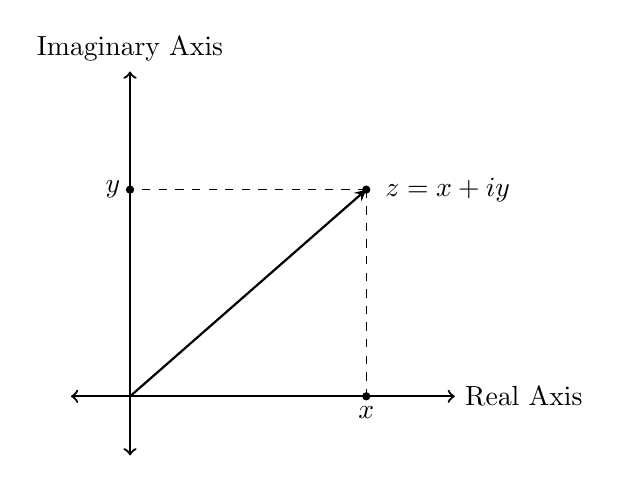
\begin{tikzpicture}[scale=0.75]
    \draw[<->,thick] (-1,0)--(5.5,0) node[right]{Real Axis};
	\draw[<->,thick] (0,-1)--(0,5.5) node[above]{Imaginary Axis};
	\draw[dashed] (4,3.5)--(0,3.5);
	\draw[dashed] (4,3.5)--(4,0);
    \fill (4,3.5) circle (2pt) node[right]{\ $z = x+iy$};
    \fill (0,3.5) circle (2pt) node[left]{$y$};
    \fill (4,0) circle (2pt) node[below]{$x$};
    \draw[->,>=stealth,thick] (0,0) -- (4,3.5);
  \end{tikzpicture}\]
Geometrically, addition of complex numbers is just the addition of the corresponding vectors in the euclidean plane. We will soon see a geometric interpretation of multiplication.

\[\begin{tikzpicture}[scale=0.75]
    \draw[<->,thick] (-1,0)--(5.5,0) node[right]{Real Axis};
	\draw[<->,thick] (0,-1)--(0,5.5) node[above]{Imaginary Axis};
    \fill[newblue] (6,4.5) circle (2pt) node[right]{\ $z_1 + z_2$};
    \fill (1,3.5) circle (2pt) node[above]{$z_1$};
    \fill (5,1) circle (2pt) node[right]{$z_2$};
    \draw[->,>=stealth,thick] (0,0) -- (1,3.5);
    \draw[->,>=stealth,thick] (0,0) -- (5,1);
	\draw[thick,dashed,newblue] (1,3.5)--(6,4.5);
	\draw[thick,dashed,newblue] (5,1)--(6,4.5);
    \draw[->,>=stealth,thick,newblue] (0,0) -- (6,4.5);
  \end{tikzpicture}\]

\medskip
 
\begin{definition}[Modulus]\label{cmplxnorm}
The \cdef{modulus} (or \cdef{absolute\ value}) of a complex number $z = x + iy$, denoted $\abs{z}$, is the length of the vector $(x,y)$, or equivalently its distance from the origin; namely
\[\abs{z} \coloneqq \sqrt{(\Re z)^2 + (\Im z)^2} = \sqrt{x^2 + y^2} = \norm{(x,y)}\]
Notice that this extends the usual absolute value of real numbers, as the modulus of a real number is its absolute value.\\[0.5em]
We can then immediately derive a useful inequality,
\[\abs{z}^2 = (\Re z)^2 + (\Im z)^2 \geq (\Re z)^2,\  (\Im z)^2,\]
giving us \[\Re z \leq \abs{\Re z} \leq \abs{z}\quad \text{and} \quad \Im z \leq \abs{\Im z} \leq \abs{z}.\]
\end{definition}

\medskip

\begin{definition}[Distance]
The \cdef{distance} between two complex numbers $z_1$ and $z_2$ is \[\abs{z_1 - z_2} = \norm{(x_1,y_1) - (x_2,y_2)} = \norm{(x_1 - x_2,y_1 - y_2)}\]
That is, it's the euclidean distance between the vectors representing these complex numbers. 
\end{definition}

\medskip

\begin{discussion}\label{firstdomain}
The absolute value can be used to define various important subsets of $\cc$.
\begin{itemize}[itemsep=1em]
\item[(1)]
\begin{itemize}[itemsep=1em]
\item[$\bullet$] The \emph{circle of radius $R>0$ centered at $z_0$} is the set
\[C_R(z_0) = \setp{z\in \cc}{\abs{z-z_0}=R}\]
\item[$\bullet$] The \emph{open disk (or ball) of radius $R>0$ centered at $z_0$} is the set
\[D_R(z_0) = \setp{z\in \cc}{\abs{z-z_0}< R}\]\\[-1em]
\[\begin{tikzpicture}[scale=0.8]
    \draw[<->,thick] (-1,0)--(5,0);
	\draw[<->,thick] (0,-1)--(0,5);
    \draw[thick,firebrick](3,3) circle (2);
    \draw[](3,3)--(4.6,4.2);
    \fill (3,3) circle (2pt);
    \node[] at (3,2.5) {$z_0$};
    \node[] at (3,5.5) {\color{firebrick}$C_R(z_0)$};
    \node[] at (3.6,4) {$R$};
  \end{tikzpicture}
  \qquad \qquad \qquad
  \begin{tikzpicture}[scale=0.8]
    \draw[<->,thick] (-1,0)--(5,0);
	\draw[<->,thick] (0,-1)--(0,5);
	\filldraw[indigo,fill opacity=1/10,dashed](3,3) circle (2);
    \draw[](3,3)--(5,3);
    \fill (3,3) circle (2pt);
    \node[] at (2.5,3) {$z_0$};
    \node[] at (3,1.75) {\color{indigo}$D_R(z_0)$};
    \node[] at (4,3.4) {$R$};
  \end{tikzpicture}\]
\item[$\bullet$] The \emph{closed disk (or ball) of radius $R>0$ centered at $z_0$} is the set
\begin{align*}
\overline{D}_R(z_0) &= \setp{z\in \cc}{\abs{z-z_0} \leq R} = D_R(z_0) \cup C_R(z_0).
\end{align*}
\end{itemize}
\item[(2)] The \emph{(open) annulus of inner radius $r>0$ and outer radius $R>0$ centered at $z_0$} is the set
\[A_{r,R}(z_0) = \setp{z\in \cc}{r < \abs{z-z_0}<R}\]\\[-1em]
\[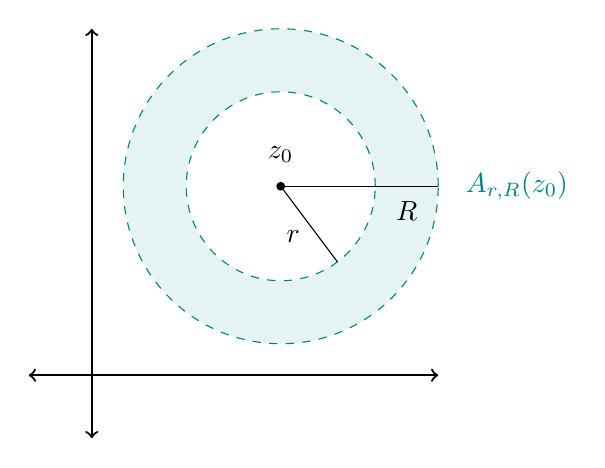
\begin{tikzpicture}[scale=0.8]
    \draw[<->,thick] (-1,0)--(5.5,0);
	\draw[<->,thick] (0,-1)--(0,5.5);
	\filldraw[teal,fill opacity=1/10,dashed](3,3) circle (2.5);
	\fill[white](3,3) circle (1.5);
    \draw[teal,dashed](3,3) circle (1.5);
    \draw[](3,3)--(5.5,3);
    \draw[](3,3)--(3.9,1.8);
    \fill (3,3) circle (2pt);
    \node[] at (3,3.5) {$z_0$};
    \node[] at (6.75,3) {\color{teal}$A_{r,R}(z_0)$};
    \node[] at (5,2.6) {$R$};
    \node[] at (3.2,2.2) {$r$};
  \end{tikzpicture}\]
\end{itemize}
\end{discussion}

%\bigskip

\begin{proposition}[Triangle Inequalities]\label{triangleineq}
For all $z_1,z_2 \in \cc$, the following inequalities hold.
\begin{itemize}
\item[(1)] $\abs{z_1 + z_2} \leq \abs{z_1} + \abs{z_2}$.
\item[(2)] $\abs{z_1 \pm z_2} \geq \abs{\abs{z_1} - \abs{z_2}}$. We sometimes refer to this inequality as the \cdef{reverse\ triangle\ inequality}.
\end{itemize}
\end{proposition}
\begin{proof}
\[\begin{tikzpicture}[scale=0.65]
    \draw[<->,thick] (-1,0)--(5.5,0);
	\draw[<->,thick] (0,-1)--(0,5.5);
    \fill[newblue] (5.5,5) circle (2pt) node[above]{\quad $z_1 + z_2$};
    \fill (0.5,3.5) circle (2pt) node[above]{$z_1$};
    \draw[->,>=stealth,thick] (0,0) -- (0.5,3.5);
    \draw[->,>=stealth,thick] (0,0) -- (5,1.5) node [pos=0.7, below,sloped] {$\abs{z_2}$};
	\draw[thick,dashed,newblue] (0.5,3.5)--(5.5,5);
	\draw[thick,newblue] (5,1.5)--(5.5,5) node [midway, right] {$\abs{z_1}$};
    \fill (5,1.5) circle (2pt) node[right]{$z_2$};
    \draw[->,>=stealth,thick,newblue] (0,0) -- (5.5,5) node [midway, above,sloped] {$\abs{z_1 + z_2}$};
  \end{tikzpicture}\]
\begin{itemize}
\item[(1)] A standard fact about triangles.
\item[(2)] We first assume that $\abs{z_1} \geq \abs{z_2}$. Then, $\abs{\abs{z_1} - \abs{z_2}} = \abs{z_1} - \abs{z_2}$. Now, note that
\begin{align*}
\abs{z_1} - \abs{z_2} &= \abs{z_1 \pm z_2 \mp z_2} - \abs{z_2}\\[0.5em]
 &\leq \abs{z_1 \pm z_2} + \abs{\mp z_2} - \abs{z_2},\ \text{triangle inequality}\\[0.5em]
 &= \abs{z_1 \pm z_2} + \abs{z_2} - \abs{z_2}\\[0.5em]
 &= \abs{z_1 \pm z_2}
\end{align*}
If we instead assume $\abs{z_2} \geq \abs{z_1}$, then we do the same computation with the roles of $z_1$ and $z_2$ switched.
\end{itemize}
\vspace*{-\baselineskip}
\end{proof}

\medskip


\begin{proposition}[Modulus is Multiplicative]\label{normmult}
\lecmargin{3}
For all $z,w \in \cc$ and positive integers $n$, 
\begin{multicols}{2}
\begin{itemize}
\item[(1)] $\abs{zw} = \abs{z}\abs{w}$.
\item[(2)] $\abs{z^n} = \abs{z}^n$.
\end{itemize}
\end{multicols}
\end{proposition}
\begin{proof}\hfill
\begin{itemize}
\item[(1)] Left as Problem \ref{prob 2.1a}. One proves these directly by showing that the left hand side matches the right hand side.
\item[(2)] The proof of this is by induction. $n = 1$ is a tautology, and $n = 2$ is (1) in the case $w = z$. Assume the statement is true for $n = k$, that is $\abs{z^k} = \abs{z}^k$. Then, for $n = k + 1$
\begin{align*}
|z^{k+1}| = |z^k\cdot z| &= |z^k|\abs{z},\quad \text{using (1)}\\[0.5em]
&= \abs{z}^k\abs{z},\quad \text{using the induction hypothesis}\\[0.5em]
&= \abs{z}^{k+1}
\end{align*}
Therefore we have the result by the principle of mathematical induction.
\end{itemize}
\vspace*{-\baselineskip}
\end{proof}

\medskip

\begin{definition}[Complex Conjugation]
Given a complex number $z = x + iy$, its \cdef{(complex)\ conjugate}, denoted $\overline{z}$, is
\[\overline{z} \coloneqq x - iy\]
Geometrically, $\overline{z}$ is the reflection of $z$ about the real axis. 
\[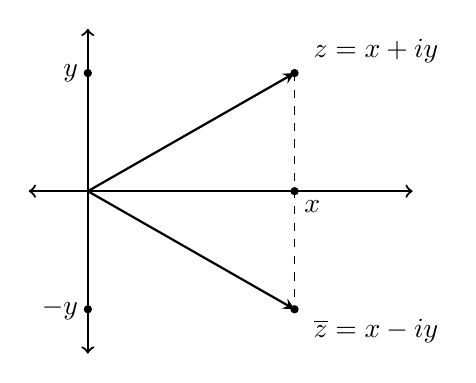
\begin{tikzpicture}[scale=0.75]
    \draw[<->,thick] (-1,0)--(5.5,0);
	\draw[<->,thick] (0,-2.75)--(0,2.75);
    \fill (3.5,2) circle (2pt) node[above right]{\ $z = x+iy$};
    \draw[->,>=stealth,thick] (0,0) -- (3.5,2);
    \fill (3.5,-2) circle (2pt) node[below right]{\ $\overline{z} = x-iy$};
    \draw[->,>=stealth,thick] (0,0) -- (3.5,-2);
    \draw[-,dashed] (3.5,2) -- (3.5,-2);
    \fill (3.5,0) circle (2pt) node[below right]{$x$};
    \fill (0,2) circle (2pt) node[left]{$y$};
    \fill (0,-2) circle (2pt) node[left]{$-y$};
  \end{tikzpicture}\]
\end{definition}

\medskip

\begin{proposition}[Properties of Conjugation]\label{conjprop}
For all pairs $z,w \in \cc$, we have
\begin{itemize}
\item[(1)] $\overline{\overline{z}} = z$
\item[(2)] $\abs{\overline{z}} = \abs{z}$
\item[(3)] $\overline{z + w} = \overline{z} + \overline{w}$
\item[(4)] $\overline{zw} = \overline{z}\ \overline{w}$
\item[(5)] $z\overline{z} = \abs{z}^2$
\item[(6)] $\Re z = \dfrac{z + \overline{z}}{2}$ and $\Im z = \dfrac{z - \overline{z}}{2i}$
\item[(7)] $z \in \rr$ if and only if $z = \overline{z}$
\end{itemize}
\end{proposition}
\begin{proof}
(1) -- (3) is clear geometrically. (4), (6) and (7) are left as Problem \ref{prob 2.1}, (7) can be proved using (6) and can also be deduced geometrically. One proves these directly by showing that the left hand side matches the right hand side.
\begin{itemize}
\item[(5)] Let $z = x + iy$, then
\begin{align*}
z\overline{z} &= (x + iy)(x - iy)\\[0.5em]
&= x^2 - ixy + iyx - i^2y^2\\[0.5em]
&= x^2 + y^2 + i(yx - xy) = x^2 + y^2 = \abs{z}^2\\[-1em]
\end{align*}
\end{itemize}
\vspace*{-\baselineskip}
\end{proof}

\medskip

\begin{discussion}
Proposition \ref{conjprop} (5) gives us a nice formula for $z^{-1}$ for $z\in \cc^*$. For such a $z$, we have $z\overline{z} = \abs{z}^2$, which gives us
\[z^{-1} = z^{-1}\cdot \frac{z\overline{z}}{\abs{z}^2} = \frac{\overline{z}}{\abs{z}^2}\]
This tells us that $z^{-1}$ is just a scaled $\overline{z}$, which means, geometrically speaking, $z^{-1}$ lies on the line passing through the origin and $\overline{z}$.
\end{discussion}

\medskip

\lecmargin{4}
Recall that every non-zero point $(x,y) \in \rr^2$ can be re-written in polar coordinates $(r,\theta)$ as
\[x = r\cos\theta \quad \text{and} \quad y = r\sin\theta\]
This suggests the following definition.
\begin{definition}[Polar Form]
If $(r,\theta)$ are polar coordinates for a non-zero $(x,y)$, then the \cdef{polar\ form} of a non-zero complex number $z = x + iy$ is
\[z = r(\cos\theta + i\sin\theta)\]
We sometimes abbreviate $\cos\theta + i\sin\theta$ as $\cis\theta$, so $z = r\cis\theta$.\\
\\
Evidently, $(r,\theta)$ are related to $(x,y)$ by the equations
\[\abs{z} = r \quad \text{and} \quad \cos\theta = \frac{x}{r} = \frac{x}{\sqrt{x^2 + y^2}},\ \sin\theta = \frac{y}{r} = \frac{y}{\sqrt{x^2 + y^2}},\ \text{so } \tan\theta = \frac{y}{x}\]
We have to be careful and take into account which quadrant $(x,y)$ belongs to, if we think of $\theta$ with respect to its formulation using $\tan$.
\[\begin{tikzpicture}[scale=0.75]
    \draw[<->,thick] (-1,0)--(5,0);
	\draw[<->,thick] (0,-1)--(0,5);
	\fill (4,3.5) circle (2pt) node[above]{\quad $z$};
    \draw[->,>=stealth,thick] (0,0) -- (4,3.5);
    \draw[|<->|,>=stealth,thick,firebrick] (-0.2478,0.2832) -- (3.752,3.783) node [fill=white, midway, sloped] {$r$};
    \draw
    (4,3.5) coordinate (a)
    -- (0,0) coordinate (b)
    -- (0.5,0) coordinate (c)
    pic["$\color{firebrick}\theta$", ->,>=stealth,thick, draw=firebrick, angle eccentricity=1.3, angle radius=1cm]
    {angle=c--b--a};
  \end{tikzpicture}\]
Since $\sin$ and $\cos$ are periodic functions, $\theta$ is not unique (you can replace $\theta$ with $\theta + 2\pi$). Each possible value of $\theta$ is called an \cdef{argument\ of} {\color{darkred}$z$}, and the set of all such $\theta$ is denoted as $\arg z$. That is, if $\theta_0$ is one solution of $\tan\theta = y/x$, then
\[\arg z = \setp{\theta_0 + 2k\pi}{k \in \zz}\]
The polar form, specifically $\theta$ is unique, as soon as we specify bounds on $\theta$. The unique argument in the interval $(-\pi,\pi]$ is called the \cdef{principal\ argument} denoted $\parg z$. Precisely speaking,
\begin{definition}\label{princ-arg}
For $z = x + iy$, we have
\[\parg z = \begin{cases}\arctan(y/x) & \text{if $x > 0$\quad \emph{\small(quadrants I \& IV)}}\\[0.5em]
\arctan(y/x) + \pi & \text{if $x < 0$ and $y > 0$\quad \emph{\small(quadrant II)}}\\[0.5em]
\arctan(y/x) - \pi & \text{if $x < 0$ and $y < 0$\quad \emph{\small(quadrant III)}}
 \end{cases}\]
\end{definition}
Notice that we can then write
\[\arg z = \setp{\parg z + 2k\pi}{k \in \zz}\]
\end{definition}

\medskip

\begin{definition}[Euler's Formula]\label{eulerform}
$e^{i\theta} \coloneqq \cis\theta = \cos\theta + i\sin\theta$. Therefore $\abs{e^{i\theta}} = 1$.
\end{definition}
\begin{proof}[Remark on Definition \ref{eulerform}]\renewcommand{\qedsymbol}{}
This is for now a stopgap, defining $e^{i\theta}$ in this way. In a few weeks, we'll see that this is truly an equality of holomorphic functions. Euler deduced this by looking at the Taylor series expansion of these functions. We haven't built or discussed enough machinery to give this reasoning a solid foundation yet. 
\end{proof}

\medskip

Using Euler's formula, one can write the polar form of a non-zero complex number, even more succinctly in its \cdef{exponential\ form}
\[z = re^{i\theta}\]
\begin{example}\hfill
\begin{itemize}[itemsep=1em]
\item[(1)] Exponential form of $1 + i$, 
\[\abs{1 + i} = \sqrt{1^2 + 1^2} = \sqrt{2}\quad \text{and} \quad \parg z = \arctan(1) = \frac{\pi}{4}\]
So, $1 + i = \sqrt{2}e^{i\pi/4}$.
\[\begin{tikzpicture}[scale=1.5]
    \draw[<-,thick] (-1.5,0)--(-1,0);
	\draw[->,thick] (0,1)--(0,1.5);
	\draw[->,thick] (1,0)--(1.5,0);
	\draw[<-,thick] (0,-1.5)--(0,-1);
	\fill[teal] (1,1) circle (0.8pt) node[above right]{\color{teal}$1+i$};
    \node (a) at (1,1) {};
    \node (b) at (0,0) {};
    \node (c) at (0.5,0) {};
    \draw pic["{\footnotesize$\color{teal}\theta = \dfrac{\pi}{4}$}", ->,>=stealth,thick, draw=teal, angle eccentricity=1.7, angle radius=1cm] {angle=c--b--a};
  \draw[->,>=stealth,teal,thick] (0,0) -- (1,1);
  \draw[->,>=stealth,firebrick,thick] (0,0) -- (1,0);
  \fill[firebrick] (1,0) circle (0.8pt) node[below]{\color{firebrick}$1$};
  \draw[->,>=stealth,firebrick,thick] (0,0) -- (0,1);
  \fill[firebrick] (0,1) circle (0.8pt) node[right]{\color{firebrick}$i$};
  \draw[->,>=stealth,firebrick,thick] (0,0) -- (-1,0);
  \fill[firebrick] (-1,0) circle (0.8pt) node[above]{\color{firebrick}$-1$};
  \draw[->,>=stealth,firebrick,thick] (0,0) -- (0,-1);
  \fill[firebrick] (0,-1) circle (0.8pt) node[left]{\color{firebrick}$-i$};
    \end{tikzpicture}\]
\item[(2)] Note that
\[1 = e^{i0} = e^{i2n\pi}\ \text{for any $n \in \zz$},\qquad i = e^{i\pi/2},\qquad -1 = e^{i\pi} = e^{i(2n+1)\pi}\ \text{for any $n \in \zz$}\]
One could write $-i = e^{i3\pi/2}$ but $3\pi/2 \neq \parg(-i)$; instead we should write $-i = e^{-i\pi/2}$.

\item[(3)] The circle $C_R(z_0)$ has a nice parametrisation 
\[C_R(z_0) = \{z = z_0 + Re^{i\theta}\ :\ 0 \leq \theta < 2\pi\}\]\\[-1.5em]
\[\begin{tikzpicture}[scale=0.75]
    \draw[<->,thick] (-1,0)--(5,0);
	\draw[<->,thick] (0,-1)--(0,5);
	\draw[->,>=stealth,thick] (0,0) -- (3,3);
    \draw[thick,indigo](3,3) circle (2);
    \draw[thick](3,3)--(5,3) node[midway, below]{$R$};
    \fill (3,3) circle (2pt);
    \node[left] at (3,3) {$z_0$};
    \draw[thick](3,3)--(2,4.732);
    \fill[indigo] (2,4.732) circle (2pt) node[above left]{$z$};
    \node (a) at (2,4.732) {};
    \node (b) at (3,3) {};
    \node (c) at (5,3) {};
    \draw pic["{\footnotesize$\theta$}", ->,>=stealth,thick,draw, angle eccentricity=1.5, angle radius=0.5cm] {angle=c--b--a};
    \node[] at (5,1) {\color{indigo}$C_R(z_0)$};
  \end{tikzpicture}\]
\end{itemize}
\vspace*{-\baselineskip}
\end{example}

\medskip

\begin{example}[in-class]
Write the exponential form of $z = 1 - i$.
\end{example}
\begin{proof}[Answer]
As a point on the plane, since $\Re z > 0$ and $\Im z < 0$, the complex number $z = 1 - i$ lies in the fourth quadrant. Thus, 
\begin{align*}
r = \abs{z} &= \sqrt{(1)^2 + (-1)^2} = \sqrt{2}\\[0.5em]
\parg z &= \arctan(-1) = -\frac{\pi}{4}
\end{align*}
Thus, $1 - i = \sqrt{2}e^{-i \pi/4}$. 
\end{proof}

\medskip

\begin{proposition}[Properties of Exponential Form]\label{propeuler}
Let $z = re^{i\theta}$ and $w = se^{i\phi}$ be non-zero complex numbers. Then
\begin{itemize}
\item[(1)] $zw = rs\  e^{i(\theta + \phi)}$
\item[(2)] $z^{-1} = (1/r) e^{-i\theta}$
\item[(3)] $z^n = r^n e^{in\theta}$, for any $n \in \zz$
\item[(4)] $\overline{z} = re^{-i\theta}$
\item[(5)] $z/w = (r/s)e^{i(\theta - \phi)}$
\end{itemize}
\end{proposition}
\begin{proof}\hfill
\begin{itemize}
\item[(1)] Note that
\begin{align*}
zw = (re^{i\theta})(se^{i\phi})&= rs(\cos\theta + i\sin\theta)(\cos\phi + i\sin\phi)\\[0.5em]
&= rs((\cos\theta\cos\phi - \sin\theta\sin\phi) + i(\cos\theta\sin\phi + \sin\theta\cos\phi))\\[0.5em]
&= rs(\cos(\theta + \phi) + i\sin(\theta + \phi))\\[0.5em]
&= rs\  e^{i(\theta + \phi)}
\end{align*}
\item[(2)] It suffices to show that $(re^{i\theta})((1/r) e^{-i\theta}) = 1$, for which we use (1).
\item[(3)] We first prove this result for $n \geq 0$, the result is clear for $n = 0$ and $n = 1$. Assume the result is true for $n = k$, that is $z^k = r^k e^{ik\theta}$. Then, for $n = k+1$
\begin{align*}
z^{k+1} &= z^kz\\[0.5em]
&= (r^k e^{ik\theta})(re^{i\theta})\ \text{using the induction hypothesis}\\[0.5em]
&= r^{k+1} e^{ik\theta+\theta}\ \text{by (1)}\\[0.5em]
&= r^{k+1} e^{i(k+1)\theta}
\end{align*}
Therefore we have the result by the principle of mathematical induction.\\[0.5em]
Suppose $n<0$ instead, then write $n = -m$ for a positive $m>0$. Now, we can apply the first case to $z^n \coloneqq (z^{-1})^m$ to get our result.
\item[(4)] Using $z\overline{z} = \abs{z}^2 = r^2$, we get that $\overline{z} = r^2z^{-1}$, and the result follows from (2).
\item[(5)] Recall $z/w = zw^{-1}$, and the result follows from (2) and (1).
\end{itemize}
\vspace*{-\baselineskip}
\end{proof}

\medskip

\begin{discussion}
Proposition \ref{propeuler} (1) gives us a nice geometric interpretation of complex multiplication. If $z = re^{i\theta}$ and $w = se^{i\phi}$, then $zw = rs\  e^{i(\theta + \phi)}$. This can be interpreted as saying that $zw$ is obtained from $w$ by scaling $w$ by $\abs{z} = r$ and rotating $w$ by an angle of $\parg z$ (or vice versa).
\[\begin{tikzpicture}
    \draw[<->,thick] (-5,0)--(5,0);
	\draw[<->,thick] (0,-1)--(0,5);
	\fill[firebrick] (2.5,1.5) circle (2pt) node[above right]{$z$};
    \draw[->,>=stealth,thick,firebrick] (0,0) -- (2.5,1.5);
    \node (a) at (2.5,1.5) {};
    \node (b) at (0,0) {};
    \node (c) at (0.2,0) {};
    \draw pic["$\color{firebrick}\theta$", ->,>=stealth,thick, draw=firebrick, angle eccentricity=1.3, angle radius=1cm] {angle=c--b--a};
    
	\fill[indigo] (0.75,3) circle (2pt) node[above]{$w$};
    \draw[->,>=stealth,thick,indigo] (0,0) -- (0.75,3);
    \node (a) at (0.75,3) {};
    \node (b) at (0,0) {};
    \node (c) at (0.2,0) {};
    \draw pic["$\color{indigo}\phi$",left, ->,>=stealth,thick, draw=indigo, angle eccentricity=2, angle radius=0.5cm] {angle=c--b--a};

	\fill[forest] (-1.5,4) circle (2pt) node[above]{$zw$};
    \draw[->,>=stealth,thick,forest] (0,0) -- (-1.5,4);
    \node (a) at (-1.5,4) {};
    \node (b) at (0,0) {};
    \node (c) at (0.2,0) {};
    \draw pic["\quad$\color{forest}\theta + \phi$", ->,>=stealth,thick, draw=forest, angle eccentricity=1.2, angle radius=1.6cm] {angle=c--b--a};
%    \draw[|<->|,>=stealth,thick] (-2.158,3.754) -- (-0.6575,-0.247) node [fill=white, midway, sloped] {$\abs{z}\abs{w}$};
    \draw [decorate,decoration={brace,amplitude=10pt,mirror,raise=4pt},yshift=0pt,thick,forest]
(-1.5,4) -- (0,0) node [black,midway,left,xshift=-0.4cm,yshift=-0.2cm] {$\color{forest}rs\ $};
  \end{tikzpicture}\]

\medskip

\begin{example}
Let's use Proposition \ref{propeuler} to compute $(1+i)^{2023}$, then
\begin{align*}
(1 + i)^{2023} &= (\sqrt{2} e^{i\pi/4})^{2023}\\[0.5em]
 &= (\sqrt{2})^{2023}(e^{i\pi/4})^{2023}\\[0.5em]
 &= (\sqrt{2})^{2022}\sqrt{2}(e^{i\pi/4})^{2024}e^{-i\pi/4}\\[0.5em]
 &= 2^{1011}\sqrt{2}(e^{i506\pi})e^{-i\pi/4}\\[0.5em]
&= 2^{1011}\sqrt{2}e^{-i\pi/4}\\[0.5em]
&= 2^{1011}(1-i)
\end{align*}
\end{example}

\medskip

\begin{example}
Compute $(1+i\sqrt{3})^{101}$.
\end{example}
\begin{proof}[Answer]
We will first compute the exponential form of our complex number. Note that \[|1 + i\sqrt{3}| = \sqrt{1^2 + (\sqrt{3})^2} = \sqrt{4} = 2,\] and since $1 + i\sqrt{3}$ lies in the first quadrant of the complex plane
\[\parg z = \arctan(\sqrt{3}) = \frac{\pi}{3}\]
Therefore
\[1+i\sqrt{3} = 2e^{i\pi/3}\]
and so
\begin{align*}
(1+i\sqrt{3})^{101} &= (2e^{i\pi/3})^{101}\\[0.5em]
 &= (2e^{i\pi/3})^{99}(2e^{i\pi/3})^{2}\\[0.5em]
 &= 2^{99}e^{i33\pi}(1+i\sqrt{3})^{2}\\[0.5em]
 &= -2^{99}(1-3 +2i\sqrt{3}),\quad \text{since $33$ is odd}\\[0.5em]
 &= -2^{99}(-2 +2i\sqrt{3})\\[0.5em]
 &= 2^{100}(1- i\sqrt{3})
\end{align*}
\end{proof}

\medskip

\lecmargin{5}
A few more interesting consequences of Proposition \ref{propeuler} are
\begin{itemize}
\item[(1)] The \emph{unit circle} \[S^1 = \setp{z\in \cc}{\abs{z} = 1} = \{e^{i\theta}\ :\ \theta \in \rr\}\] is closed under multiplication. It's in fact an abelian group, usually denoted $U(1)$.
\item[(2)] \emph{De Moivre's Theorem}. From Proposition \ref{propeuler} (4) applied to $z = e^{i\theta}$ we get
\[(\cos\theta + i\sin\theta)^n = (\cos n\theta + i\sin n\theta)\]
\end{itemize}
\vspace*{-\baselineskip}
\end{discussion}

\medskip

\begin{proposition}[Arguments of Products]\label{prodarg}
Let $z,w$ be non-zero complex numbers, then
\begin{itemize}
\item[(1)] $\arg (zw) = \arg z + \arg w$
\item[(2)] $\arg w^{-1} = -\arg w$
\end{itemize}
\emph{Note that this is \emph{not} saying $\parg(zw) = \parg z + \parg w$, this is actually not true, we're claiming an equality of sets. (1) and (2) together give us $\arg (z/w) = \arg z - \arg w$.}
\end{proposition}
\begin{proof}\hfill
\begin{itemize}
\item[(1)] Consider $\theta \in \arg z$ and $\phi \in \arg w$, so $z = re^{i\theta}$ and $w = se^{i\phi}$. By Proposition \ref{propeuler} (1), we have $zw = rs\ e^{i(\theta + \phi)}$ and therefore $\theta + \phi \in \arg(zw)$. Hence $\arg z + \arg w \subseteq \arg(z + w)$.\\[0.5em]
Consider $\psi \in \arg(z+w)$, and some $\theta \in \arg z$ then we claim that $\psi - \theta \in \arg w$. We have $rs\ e^{i\psi} = zw = re^{i\theta}w$, then by Proposition \ref{propeuler} (5), we get $w = sr^{i(\psi - \theta)}$. Hence $\psi - \theta \in \arg w$, and since $\psi = \theta + (\psi - \theta) \in \arg z + \arg w$, we have $\arg(z+w) \subseteq \arg z + \arg w$.\\[0.5em]
Therefore $\arg (zw) = \arg z + \arg w$.
\item[(2)] Consider $\theta \in \arg z$, so $z = re^{i\theta}$. By Proposition \ref{propeuler} (2), we have $z^{-1} = (1/r)e^{i(-\theta)}$ and therefore $-\theta \in \arg w^{-1}$. Hence $-\arg w \subseteq \arg w^{-1}$.\\[0.5em]
Note that $w = (w^{-1})^{-1}$, applying the above result to $w^{-1}$ gets us $-\arg w^{-1} \subseteq \arg (w^{-1})^{-1} = \arg w$ and so $\arg w^{-1} \subseteq - \arg w$.\\[0.5em]
Therefore $\arg w^{-1} = -\arg w$.
\end{itemize}
\vspace*{-\baselineskip}
\end{proof}

\medskip

\begin{remark}
For a complex number, $\arg z$ is a set of all possible $\theta$'s such that we can write $z = \abs{z}e^{i\theta}$, as you know. Therefore, we will abuse notation by sometimes calling any $\theta \in \arg z$ as an argument of $z$, and sometimes also writing $z = \abs{z}e^{i\arg z}$. That is, we are not, or are careless about, distinguishing the set $\arg z$ and its element when we can be agnostic about the choice of $\theta$; for example, the polar form of a complex number. It will be clear when we choose to care about out choice, it will be evident because we'll be then forcing $\theta$ to lie in an interval of length $2\pi$; for example, the principal argument $-\pi < \parg z \leq \pi$.
\end{remark}

\medskip

\begin{example}\hfill
\begin{itemize}
\item[(1)] The principal argument of $z = (\sqrt{3} - i)^6$. We first note that $\parg(\sqrt{3} - i) = -\pi/6$. By Proposition \ref{prodarg} (1), applied inductively, we have
\begin{align*}
\arg (\sqrt{3} - i)^6 &= \underbrace{\arg(\sqrt{3} - i) + \cdots + \arg(\sqrt{3} - i)}_{\text{$6$ times}} = \setp{-\pi + 2k\pi}{k \in \zz}
\end{align*}
Then $\parg(\sqrt{3} - i)^6$ is the element in the set above in the interval $(-\pi,\pi]$ which is $\pi$.
\item[(2)] As mentioned previously, we can't just replace $\arg$ with $\parg$ in the statement of Proposition \ref{prodarg} (1). Here's a simple example: let $z = w = -1$, then $\parg z = \parg w = \pi$ and $\parg zw = \parg 1 = 0$ but $0 \neq 2\pi = \parg z + \parg w$.
\item[(3)] Note that $\arg z + \arg z \neq 2\arg z$.
\end{itemize}
\vspace*{-\baselineskip}
\end{example}

\bigskip

\subsection{Roots of Complex Numbers}
%\begin{mdframed}
%\begin{center}
%{\Large Roots of Complex Numbers}
%\end{center}
%\end{mdframed}

\begin{lemma}\label{polareq}
Two non-zero complex numbers $z,w$ are equal if and only if $\abs{z} = \abs{w}$ and $\arg z = \arg w$.
\end{lemma}
\begin{proof}
If $\abs{z} = \abs{w}$ and $\arg z = \arg w$, then clearly $z = w$.\\[0.5em]
Suppose $z = w$, then we immediately get $\abs{z} = \abs{w}$. Consider $\theta \in \arg z$ and $\phi \in \arg w$, then we get $e^{i\theta} = e^{i\phi}$ which is equivalent to saying $\cos(\theta - \phi) + i\sin(\theta - \phi) = e^{i(\theta - \phi)} = 1$. This gives us
\[\sin (\theta - \phi) = 0.\]
The solution to this is $\theta - \phi = 2k\pi$ for some $k\in \zz$. This gives us $\arg z = \arg w$.
\end{proof}

\medskip

\begin{definition}[Roots]
\lecmargin{6}
Let $\alpha$ be a non-zero complex number. An \emph{$n^{\text{th}}$ root of $\alpha$} is a solution to the polynomial equation $z^n - \alpha = 0$.\\
\\
The set of all $n^{\text{th}}$ roots of $\alpha$ is denoted by $\alpha^{1/n}$, we reserve the symbol $\sqrt[n]{\ \cdot\ }$ for the unique positive $n^{\text{th}}$ root of a positive real number.
\end{definition}

\medskip

\begin{proposition}[Distinct Roots]\label{distroot}
There are precisely $n$ distinct $n^{\text{th}}$ roots of $\alpha$, namely
\[\beta_k = \sqrt[n]{\abs{\alpha}}\ e^{i\left(\frac{\parg \alpha}{n} + \frac{2k\pi}{n}\right)},\quad k = 0,\ldots,n-1\]
\end{proposition}
\begin{proof}
Let $z = re^{i\theta}$ and $\alpha = \abs{\alpha}e^{i\parg\alpha}$, we solve
\[r^ne^{in\theta} = z^n = \alpha = \abs{\alpha}e^{i\parg\alpha}.\]
By Lemma \ref{polareq}, this equality is true if and only if $r^n = \abs{\alpha}$ and $n\theta = \parg\alpha + 2k\pi$ for some $k \in \zz$. Therefore
\[z = \sqrt[n]{\abs{\alpha}}\ e^{i\left(\frac{\parg \alpha}{n} + \frac{2k\pi}{n}\right)},\quad k \in \zz\]
We obtain distinct $n$ complex numbers for $k = 0,\ldots,n-1$ since they have distinct arguments, and they necessarily give us the $n$ distinct $n^{\text{th}}$ roots of $\alpha$.
\end{proof}

\medskip

\begin{discussion}
With the notation of Proposition \ref{distroot}, the {\color{darkred}$n^{\text{th}}$} \cdef{principal\ root\ of} {\color{darkred}$\alpha$} is
\[\beta_0 = \sqrt[n]{\abs{\alpha}}\ e^{i\frac{\parg \alpha}{n}}\]
If we introduce the notation $\zeta_n = e^{\frac{2\pi i}{n}}$, then
\[\zeta_n^k = e^{\frac{2k\pi i}{n}}\]
According to the proposition, the complex numbers
\[1,\ \zeta_n,\ \zeta_n^2,\ldots,\zeta_n^{n-1}\]
are the distinct solutions to $z^n - 1 = 0$, the {\color{darkred}$n^{\text{th}}$} \cdef{roots\ of\ unity}, making $\zeta_n$ the \cdef{primitive} \emph{$n^{\text{th}}$ root of unity} as it generates all $n^{\text{th}}$ other roots of unity.\\
\\
Then we can write the roots of $\alpha$ in terms of the principal root and the primitive root of unity
\begin{align*}
\beta_k &= \sqrt[n]{\abs{\alpha}}\ e^{i\left(\frac{\parg \alpha}{n} + \frac{2k\pi}{n}\right)}\\[0.5em]
 &= \sqrt[n]{\abs{\alpha}}\ e^{i\frac{\parg \alpha}{n}}e^{\frac{2k\pi i}{n}}  = \beta_0\zeta_n^k
\end{align*}
That is, $\beta_k$'s all lie on the circle of radius $\sqrt[n]{\abs{\alpha}}$ centered at the origin, and all of them are obtained by rotating $\beta_0$ by an angle of $2k\pi/n$. That is, they all lie on the vertices of an inscribed regular $n$-gon.
\[\begin{tikzpicture}
    \draw[<->,thick] (-2.5,0)--(2.5,0);
	\draw[<->,thick] (0,-3)--(0,3);
    \draw[thick](0,0) circle (2);
    \draw[->,>=stealth,thick,firebrick](0,0)--(-0.41,1.958);
    \draw[->,>=stealth,thick,firebrick](0,0)--(-1.4,1.428);
    \fill[firebrick] (-0.41,1.958) circle (2pt) node[above]{\color{firebrick}$\beta_{k-1}$};
    \fill[firebrick] (-1.4,1.428) circle (2pt) node[above left]{\color{firebrick}$\beta_{k}$};
    \node (a) at (-1.4,1.428) {};
    \node (b) at (0,0) {};
    \node (c) at (-0.41,1.958) {};
    \draw[->,>=stealth,thick,firebrick](0,0)--(1.73,1.004) node[midway,above,sloped]{\color{firebrick}$\sqrt[n]{\abs{\alpha}}$};
    \fill[firebrick] (1.73,1.004) circle (2pt) node[above right]{\color{firebrick}$\beta_0$};
    \draw pic["{\scriptsize$\color{firebrick}\ \dfrac{2\pi}{n}$}", ->,>=stealth,thick,draw=firebrick, angle eccentricity=1.4, angle radius=1cm] {angle=c--b--a};
  \end{tikzpicture}\]
\end{discussion}

\medskip

\begin{example}\hfill
\begin{itemize}
\item[(1)] We compute explicitly the $4^{\text{th}}$ roots of $\alpha = -16$. As a negative real number, $\parg(-16) = \pi$, so
\begin{align*}
\beta_k &= \sqrt[4]{16}e^{i\left(\frac{\pi}{4}+\frac{2k\pi}{4}\right)} = 2\ e^{i\frac{\pi}{4}}e^{\frac{ki\pi}{2}}\\[0.5em]
&= 2\ e^{i\frac{\pi}{4}}\left(e^{\frac{i\pi}{2}}\right)^k\\[0.5em]
&= 2\ \left(\cos\frac{\pi}{4} + i\sin\frac{\pi}{4}\right)\left(\cos\frac{\pi}{2} + i\sin\frac{\pi}{2}\right)^k = 2\ \left(\frac{1}{\sqrt{2}} + i\frac{1}{\sqrt{2}}\right)i^k = \sqrt{2}(1 + i)i^k
\end{align*}
Therefore
\[\begin{tikzpicture}
    \draw[<->,thick] (-2.5,0)--(2.5,0);
	\draw[<->,thick] (0,-2.5)--(0,2.5);
    \draw[thick](0,0) circle (2);
    \draw[->,>=stealth,thick,indigo](0,0)--(1.414,1.414) node[above, midway, sloped]{\color{indigo}$2$};
    \draw[thick,indigo,dashed](1.414,1.414)--(1.414,-1.414);
    \draw[thick,indigo,dashed](1.414,-1.414)--(-1.414,-1.414);
    \draw[thick,indigo,dashed](-1.414,-1.414)--(-1.414,1.414);
    \draw[thick,indigo,dashed](-1.414,1.414)--(1.414,1.414);
    \fill[indigo] (1.414,1.414) circle (2pt) node[above right]{\color{indigo}$\sqrt{2}(1 + i)$};
    \fill[indigo] (1.414,-1.414) circle (2pt) node[below right]{\color{indigo}$\sqrt{2}(1 - i)$};
    \fill[indigo] (-1.414,1.414) circle (2pt) node[above left]{\color{indigo}$\sqrt{2}(-1 + i)$};
    \fill[indigo] (-1.414,-1.414) circle (2pt) node[below left]{\color{indigo}$\sqrt{2}(-1 - i)$};
    \node (a) at (1.414,1.414) {};
    \node (b) at (0,0) {};
    \node (c) at (2,0) {};
    \draw pic["{\scriptsize$\color{indigo}\ \dfrac{\pi}{4}$}", ->,>=stealth,thick,draw=indigo, angle eccentricity=1.25, angle radius=1cm] {angle=c--b--a};
  \end{tikzpicture}\]
\[\beta_0 = \sqrt{2}(1 + i),\quad \beta_1 = \sqrt{2}(-1 + i),\quad \beta_2 = \sqrt{2}(-1-i),\quad \beta_3 = \sqrt{2}(1-i)\]
\item[(2)] In the course of the previous example, we have computed the $4^{\text{th}}$ roots of unity, since they are
\[e^{\frac{2ki\pi}{4}} = e^{\frac{ki\pi}{2}},\quad k = 0,1,2,3\]
as $\parg 1 = 0$. Letting $\zeta_4 = e^{i\pi/2} = i$, the $4^{\text{th}}$ roots of unity are $\zeta_4^0,\zeta_4^1,\zeta_4^2,\zeta_4^3$, which are nothing but $\pm 1,\pm i$. Furthermore, note that $i$ is the primitive $4^{\text{th}}$ root of unity. 
\end{itemize}
\end{example}

\medskip

\begin{example}\label{cuberootofunity}
\lecmargin{7}
We compute the $3^{\text{rd}}$ roots of unity, also called the cube roots of unity where we denote $\omega = \zeta_3$, explicitly.
\[\begin{tikzpicture}[scale=0.8]
    \draw[<->,thick] (-3,0)--(3,0);
	\draw[<->,thick] (0,-3)--(0,3);
    \draw[thick](0,0) circle (2);
    \draw[->,>=stealth,thick,dirt](0,0)--(-1,1.732);
    \draw[thick,dirt,dashed](2,0)--(-1,1.732);
    \draw[thick,dirt,dashed](-1,1.732)--(-1,-1.732);
    \draw[thick,dirt,dashed](-1,-1.732)--(2,0);
    \fill[dirt] (-1,1.732) circle (2pt) node[above left]{\color{dirt}$\omega$};
    \fill[dirt] (-1,-1.732) circle (2pt) node[below left]{\color{dirt}$\omega^2$};
    \fill[dirt] (2,0) circle (2pt) node[below right]{\color{dirt}$1$};
    \node (a) at (-1,1.732) {};
    \node (b) at (0,0) {};
    \node (c) at (2,0) {};
    \draw pic["{\ \ \tiny$\color{dirt}\ \dfrac{2\pi}{3}$}", ->,>=stealth,thick,draw=dirt, angle eccentricity=1.6, angle radius=0.3cm] {angle=c--b--a};
  \end{tikzpicture}\]
Let the primitive root be $\omega = \zeta_3$, then the cube roots of unity are
\[1,\ \omega,\ \omega^2\]
where we have
\begin{align*}
\omega = e^{\frac{2\pi i}{3}} &= \left(\cos\frac{2\pi}{3} + i\sin\frac{2\pi}{3}\right) = -\frac{1}{2}+i\frac{\sqrt{3}}{2}\\[0.5em]
\omega^2 = e^{\frac{4\pi i}{3}} &= \left(\cos\frac{4\pi}{3} + i\sin\frac{4\pi}{3}\right) = -\frac{1}{2}-i\frac{\sqrt{3}}{2}
\end{align*}
\end{example}

\bigskip

\subsection{Basic Topology of $\cc$}
%\begin{mdframed}
%\begin{center}
%{\Large Basic Topology of $\cc$}
%\end{center}
%\end{mdframed}

Our purpose now is to define the kind of subsets of $\cc$ that are suitable for doing complex analysis, namely \emph{non-empty open connected sets}.
\begin{definition}[Open Disks or Neighbourhoods]
Let $\epsilon>0$. Recall the \cdef{open\ disk} (of radius $\epsilon$ centered at $z_0$) is the set
\[D_\epsilon(z_0) = \setp{z\in \cc}{\abs{z - z_0}<\epsilon}.\]
We also refer to such an open disk as an {\color{darkred}$\epsilon$-}\cdef{neighbourhood} or simply a \cdef{neighbourhood}.\\
\\
A \cdef{deleted} (or \cdef{punctured}) \cdef{open\ disk} (or \cdef{neighbourhood}) is a set of the form
\[D_\epsilon(z_0)\setminus\set{z_0} = \setp{z\in \cc}{0 < \abs{z - z_0}<\epsilon}.\]\\[-0.5em]
\[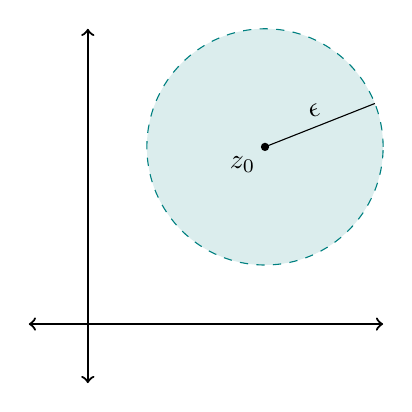
\begin{tikzpicture}[scale=0.75]
    \draw[<->,thick] (-1,0)--(5,0);
	\draw[<->,thick] (0,-1)--(0,5);
	\filldraw[teal,fill opacity=1/7,dashed](3,3) circle (2);
    \draw[](3,3)--(4.86,3.735) node[sloped,midway,above]{$\epsilon$};
    \fill (3,3) circle (2pt) node[below left]{$z_0$};
  \end{tikzpicture}
  \qquad\qquad\qquad
  \begin{tikzpicture}[scale=0.75]
    \draw[<->,thick] (-1,0)--(5,0);
	\draw[<->,thick] (0,-1)--(0,5);
	\filldraw[forest,fill opacity=1/7,dashed](3,3) circle (2);
    \draw[forest,dotted](3,3) circle (3pt);    
    \draw[](3,3)--(4.86,3.735) node[sloped,midway,above]{$\epsilon$};
    \fill[white] (3,3) circle (3pt) node[below left]{\color{black}$z_0$};
  \end{tikzpicture}\]
Points belonging to the same $\epsilon$-neighbourhood are considered "close" to each other, in the sense that they are within a distance of $2\epsilon$ from each other.
\end{definition}

\medskip

\begin{definition}[Various kinds of Points]
Consider a $S \subseteq \cc$. 
\begin{itemize}
\item A point $z \in S$ is an \cdef{interior\ point\ of} {\color{darkred}$S$} if there exists an $\epsilon > 0$ such that $D_\epsilon(z) \subseteq S$. 
\item A point $z \notin S$ is an \cdef{exterior\ point\ of} {\color{darkred}$S$} if there exists an $\epsilon > 0$ such that $D_\epsilon(z) \cap S = \emptyset$. 
\item A point $z \in \cc$ is a \cdef{boundary\ point\ of} {\color{darkred}$S$} if it's neither an interior nor an exterior point of $S$. Equivalently, if every neighbourhood of $z$ contains both a point in $S$ and not in $S$.
\item A point $z \in \cc$ is a \cdef{accumulation} (or \cdef{cluster}) \cdef{point\ of} {\color{darkred}$S$} if for every $\epsilon > 0$ we have \[D_\epsilon(z)\setminus\set{z} \cap S \neq \emptyset.\]
\item A point $z \in S$ is an \cdef{isolated\ point\ of} {\color{darkred}$S$} if there exists an $\epsilon > 0$ such that $D_\epsilon(z)\setminus\set{z} \cap S = \emptyset$. Isolated points are examples of boundary point
\end{itemize}
\[\begin{tikzpicture}[scale=1.1]
    \draw[<->,thick] (-2,0)--(5,0);
	\draw[<->,thick] (0,-2)--(0,5);
    \node[] at (4.75,2) {\color{dirt}$S$};
    
    \fill (3,4) circle (2pt) node[below]{\scriptsize$z_1$};
    \draw[](3,4)--(3.4,4.3) node[sloped,midway,xshift=-1pt,yshift=4pt]{\tiny$\epsilon_1$};
    \filldraw[indigo,fill opacity=1/10,dashed](3,4) circle (0.5);
    
    \fill (2.7,0.85) circle (2pt) node[below]{\scriptsize$z_2$};
    \draw[](2.7,0.85)--(3.45,0.85) node[sloped,midway,above,yshift=-1pt]{\tiny$\epsilon_2$};
    \filldraw[newblue,fill opacity=1/10,dashed](2.7,0.85) circle (0.75);
    
    \fill (-0.75,3.25) circle (2pt) node[below]{\scriptsize$z_3$};
    \draw[](-0.75,3.25)--(-1.75,3.25) node[sloped,midway,above,yshift=-1pt]{\tiny$\epsilon_3$};
    \filldraw[firebrick,fill opacity=1/10,dashed](-0.75,3.25) circle (1);
    
    \path[draw,use Hobby shortcut,closed=true,fill=dirt,fill opacity=1/10,dashed]
(-1,0) .. (3,0) .. (3,4) .. (1.5,2) .. (-1,0);
	\fill[dirt] (5,3) circle (2pt) node[below]{\scriptsize$z_4$};
\end{tikzpicture}\]
Here $z_1$ is a boundary point, $z_2$ an interior point, $z_3$ an exterior point, and $z_4$ is an isolated point (and a boundary point).
\end{definition}

%\medskip

\begin{remark}
The idea is that if we don't move too far from an interior point of $S$ then we remain in $S$; a similar idea holds for an exterior point. But at a boundary point we can make an arbitrarily small move and get to a point inside $S$, and we can also make an arbitrarily small move and get to a point outside $S$. An accumulation point is one where it has other points from $S$ within any arbitrarily small distance, i.e. points "accumulate" near it; an isolated point is the exact opposite.
\end{remark}

\medskip

\begin{definition}[Open and Closed Sets]
Consider a $S \subseteq \cc$.
\begin{itemize}
\item The \cdef{interior\ of} {\color{darkred}$S$} is the set of all interior points of $S$, denoted $S^\circ$.
\item $S$ is said to be \cdef{open} if $S = S^\circ$.
\item The \cdef{boundary\ of} {\color{darkred}$S$} is the set of all boundary points of $S$, denoted $\partial S$.
\item $S$ is said to be \cdef{closed} if $\partial S \subseteq S$. Equivalently, if its complement is open.
\item The \cdef{closure\ of} {\color{darkred}$S$} is the set $S \cup \partial S$, denoted $\overline{S}$.
\end{itemize}
\end{definition}

\medskip

\begin{example}\hfill
\begin{itemize}
\item[(1)] The open disks $D_R(z_0)$ are truly open sets, and the closed disks $\overline{D}_R(z_0)$ are truly closed sets.\\[0.5em]
The closure of the open disk $D_R(z_0)$ is $\overline{D}_R(z_0)$. The boundary of $D_R(z_0)$ is the circle $C_R(z_0)$.
\item[(2)] Consider the upper half-plane 
\[\mathbf{H} = \setp{z\in \cc}{\Im z>0},\]
then we have $\mathbf{H}^\circ = \mathbf{H}$. Since by definition $\mathbf{H}^\circ \subseteq \mathbf{H}$, it's enough to prove $\mathbf{H} \subseteq \mathbf{H}^\circ$. Consider any $z \in \mathbf{H}$, then $\Im z > 0$. Let $\epsilon = (\Im z)/2$, we claim that
\[D_\epsilon(z) \subseteq \mathbf{H}\]\\[-1em]
\[\begin{tikzpicture}[scale=0.9]
    \draw[<->,thick] (-5,0)--(5,0);
	\draw[<->,thick] (0,-2)--(0,5.5);
    \node[] at (5.5,2.25) {\color{dirt}$\mathbf{H}$};
	\draw[dashed,dirt] (-5,5)--(5,5);
    \fill[dirt,fill opacity=1/10](-5,0) -- (-5,5) -- (5,5) -- (5,0);
    
    \fill (2,3) circle (2pt) node[above]{\footnotesize$z$};
    \draw[](2,3)--(2,1.5) node[midway,right]{\tiny$\dfrac{\Im z}{2}$};
    \filldraw[newblue,fill opacity=1/10,dashed](2,3) circle (1.5);
  \end{tikzpicture}\]
\lecmargin{8}
Let $w \in D_\epsilon(z)$, then \[\abs{w - z} < \epsilon = \frac{\Im z}{2}\]
The end of Discussion \ref{cmplxnorm} tells us
\begin{align*}
\frac{\Im z}{2} > \abs{w - z} &\geq \abs{\Im(w - z)}\\[0.5em]
&= \abs{\Im w - \Im z}
\end{align*}
The later is simply the absolute value of a real number, which gives
\[-\frac{\Im z}{2} < \Im w - \Im z < \frac{\Im z}{2}\]
Adding $\Im z$ throughout the inequality, we get from the inequality on the left hand side
\[\Im w > \frac{\Im z}{2} > 0.\]
Therefore $w \in \mathbf{H}$, and hence $D_\epsilon(z) \subseteq \mathbf{H}$. Thus $\mathbf{H}^\circ = \mathbf{H}$.\\[1em]
The points exterior to $\mathbf{H}$ are points $z$ such that $\Im z < 0$. That is, the exterior of the upper half-plane is the (open) lower half-plane. The boundary of $\mathbf{H}$ consists of precisely points $z$ whose $\Im z = 0$. That is, $\partial \mathbf{H} = \rr$.\\[0.5em]
The closure of $\mathbf{H}$ is $\overline{\mathbf{H}} = \setp{z\in \cc}{\Im z\geq 0}$. While $\mathbf{H} \cup \set{0}$ is neither open nor closed.
\end{itemize}
\end{example}

\medskip

\begin{definition}[Bounded Sets]
A set $S \subseteq \cc$ is \cdef{bounded} if $S \subseteq D_M(0)$ for some $M>0$. That is, there exists an $M>0$ such that $\abs{z} \leq M$ for every $z \in S$.
\end{definition}

\medskip

\begin{definition}[Connected Sets]
A set $S \subseteq \cc$ is said to be \cdef{connected} if each pair of points $z_1$ and $z_2$ in $S$ can be joined by a \emph{polygonal line}, consisting of a finite number of line segments joined end to end, that lies entirely in $S$. Otherwise, we say it is \cdef{disconnected}.
\[\begin{tikzpicture}[scale=0.75]
    \draw[<->,thick] (-2,0)--(5,0);
	\draw[<->,thick] (0,-2)--(0,5);
    \node[] at (4,4) {\color{dirt}$S$};
    \path[draw,use Hobby shortcut,closed=true,fill=dirt,fill opacity=1/10,dashed]
%(-1,0) .. (3,0) .. (3,4) .. (1.5,2) .. (-1,0);
(-2,4) .. (1,2) .. (4,3.5) .. (6,1) .. (5,2) .. (3,0) .. (1.5,-1) .. (1,0) .. (0,1) .. (-2,4);
    \draw[](-1.5,3.5)--(1.5,1);
    \draw[](1.5,1)--(5.5,3.5);
    \draw[](5.5,3.5)--(6.25,2);
    \fill (-1.5,3.5) circle (2pt) node[below left]{$z_1$};
    \fill (6.25,2) circle (2pt) node[below right]{$z_2$};
%    \fill (1.5,1) circle (2pt);
%    \fill (5.5,3.5) circle (2pt);
\end{tikzpicture}\]
\end{definition}

\medskip

\begin{definition}[Domain]
$S \subseteq \cc$ is called a \cdef{domain} if it's a non-empty open and connected set.\\[0.5em]
A \cdef{region} is a domain together with some or all of its boundary points.
\end{definition}

\medskip

\begin{remark}
Domains and regions are sets we will find most suitable for stating elegant results about certain functions in a complex variable.
\end{remark}

\medskip

\begin{example}
$\mathbf{H}$ is a domain since it's non-empty, open and any two points in $\mathbf{H}$ can be connected by a straight line. It's an unbounded set. An example of a region is $\mathbf{H} \cup \set{0}$.
\end{example}